\documentclass{standalone}
\usepackage{tikz,tikz-3dplot}
\usetikzlibrary{perspective,patterns}
\usetikzlibrary{calc,fadings,decorations.pathreplacing}
\usetikzlibrary{shapes,fit}
\usetikzlibrary{hobby}
\usetikzlibrary{arrows.meta}
\begin{document}
\tikzset{illustration/.style={very thin}}
\tikzset{dimension/.style={very thin,lightgray}}
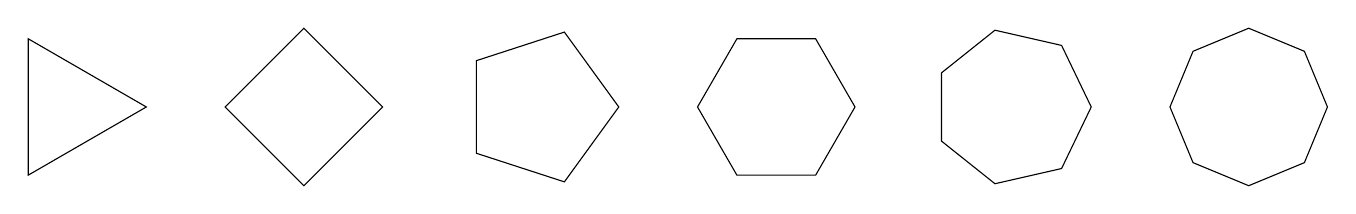
\begin{tikzpicture}[]
\draw (4.0,0.0)--(2.5,0.866)--(2.5,-0.866)--cycle;
\draw (7.0,0.0)--(6.0,1.0)--(5.0,0)--(6.0,-1.0)--cycle;
\draw (10.0,0.0)--(9.309,0.9511)--(8.191,0.5878)--(8.191,-0.5878)--(9.309,-0.9511)--cycle;
\draw (13.0,0.0)--(12.5,0.866)--(11.5,0.866)--(11.0,0)--(11.5,-0.866)--(12.5,-0.866)--cycle;
\draw (16.0,0.0)--(15.6235,0.7818)--(14.7775,0.9749)--(14.099,0.4339)--(14.099,-0.4339)--(14.7775,-0.9749)--(15.6235,-0.7818)--cycle;
\draw (19.0,0.0)--(18.7071,0.7071)--(18.0,1.0)--(17.2929,0.7071)--(17.0,0)--(17.2929,-0.7071)--(18.0,-1.0)--(18.7071,-0.7071)--cycle;
\end{tikzpicture}
\end{document}
